%%
%% Created in 2018 by Martin Slapak
%%
%% Based on file for NRP report LaTeX class by Vit Zyka (2008)
%%
%% Compilation:
%% >pdflatex report
%% >bibtex report
%% >pdflatex report
%% >pdflatex report

\documentclass[czech]{mvi-report}

\usepackage[utf8]{inputenc}
\usepackage{amsmath}
\usepackage{colortbl}
\usepackage{listings}

\usepackage{graphicx}
\graphicspath{ {./img/} }

\title{DÚ č.2 - Testování hypotéz}

\author{Marek Nevole, Jan Novotný}
\affiliation{ČVUT - FIT}
\email{\{nevolmar, novot103\}@fit.cvut.cz}

\def\file#1{{\tt#1}}

\begin{document}

\maketitle

%%%%%%%%%%%%%%%%%%%%%%%%%%%%%%%%%%%%%%%%%%%%%%%%%%%%%%%%%%%%%%%%%%%%%%%%%%%%%%%%
\section{Úvod}
Ve druhém úkolu z předmětu vybrané statistické metody jsme se zabývali testováním hypotéz a testy nezávislosti. Za reprezentanta byl zvolen Marek Nevole.

\begin{align*}
  K &= 28\\
  L &= 6\\
  X &= ((23KL)\text{ mod }20) + 1\\
  X &= 5\\
  Y &= ((X + ((5K + 7L)\text{ mod }19))\text{ mod }20) + 1\\
  Y &= 17
\end{align*}

Výsledkem těchto rovnic jsou názvy vybraných datových souborů. V našem případě budeme pracovat se soubory 005.txt a 017.txt.

Úkol jsme vypracovali pomocí programovacího jazyka Python\footnote{python.org} v prostředí Jupyter Notebook\footnote{jupyter.org} s volně dostupnými knihovnami SciPy\footnote{scipy.org}, NumPy\footnote{numpy.org} a Matplotlib\footnote{matplotlib.org}.

\section{Úloha č.1}
\textit{Z obou datových souborů načtěte texty k analýze. Pro každý text zvlášť odhadněte základní charakteristiky délek slov, tj. střední hodnotu a rozptyl. Graficky znázorněte rozdělení délek slov.}\\



\begin{figure}
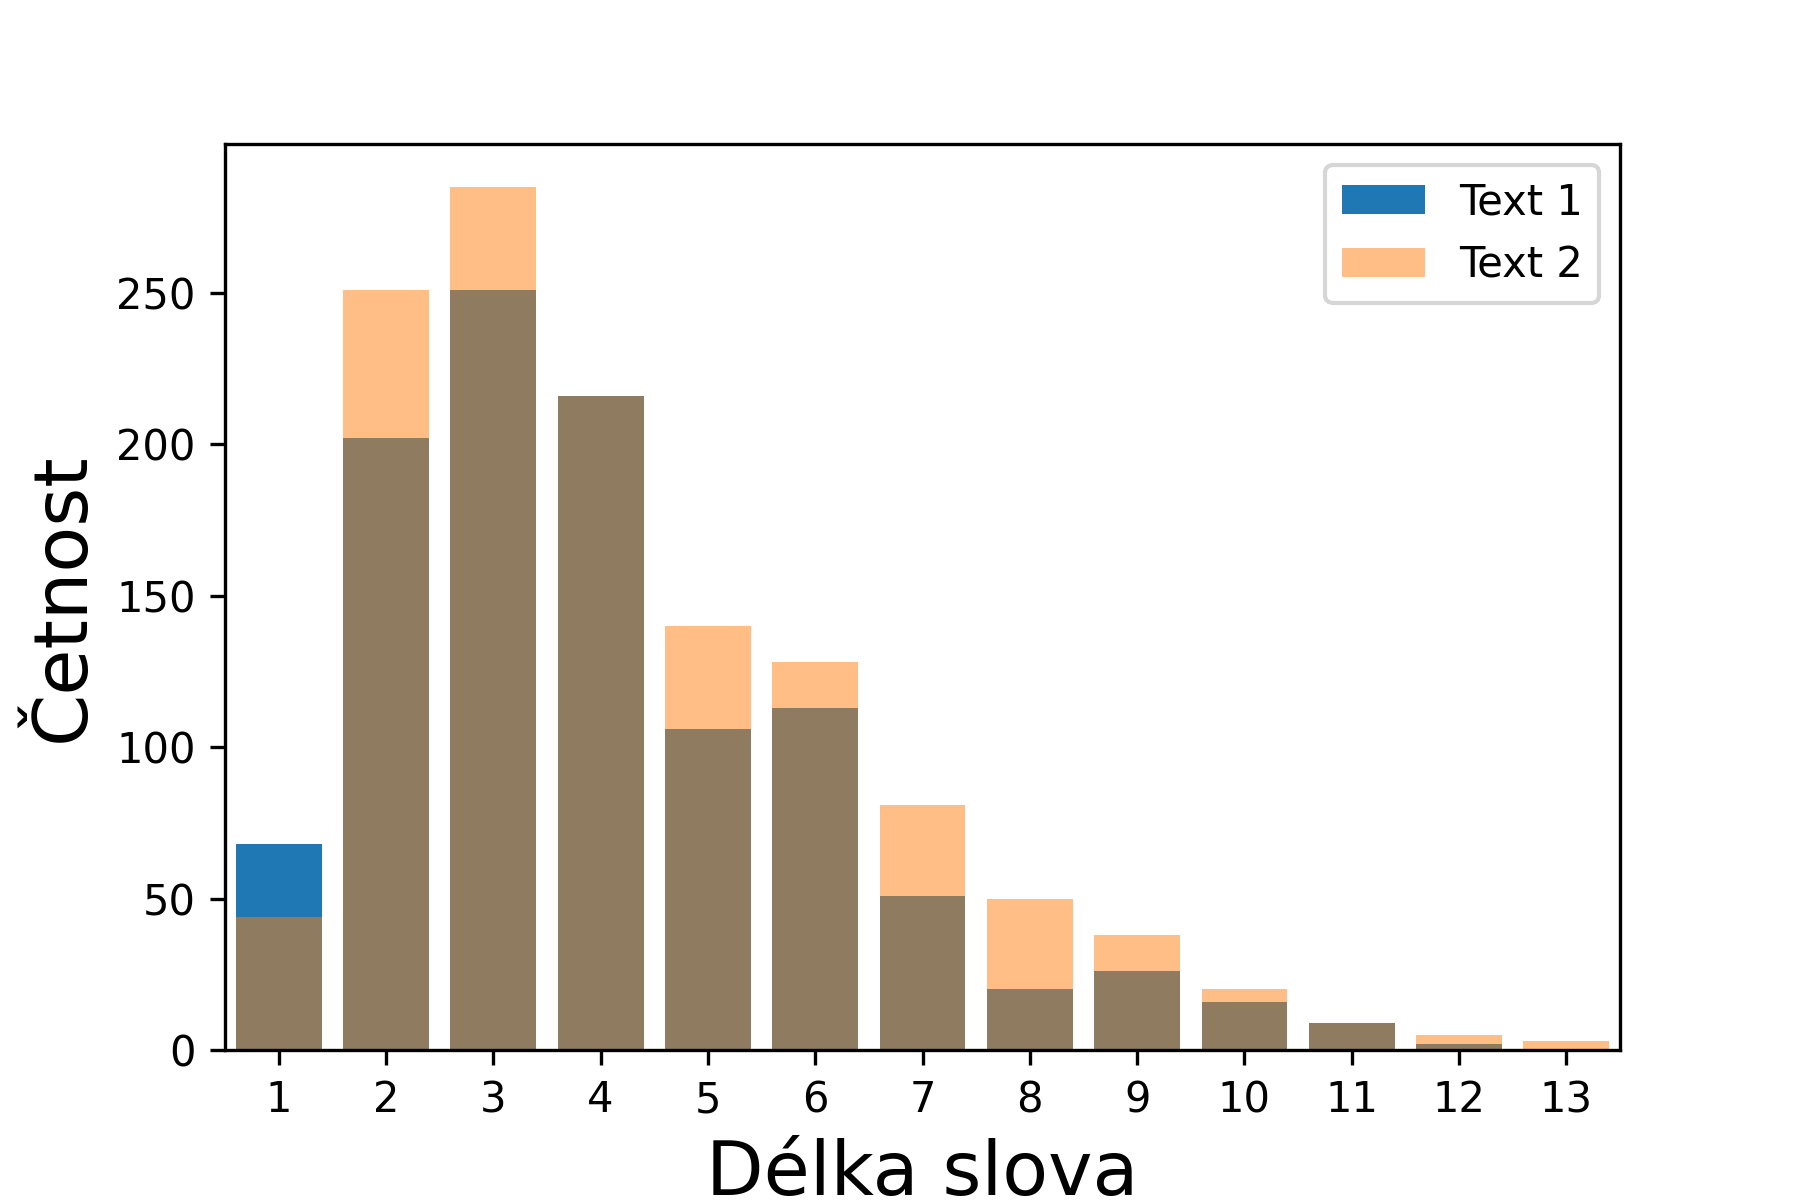
\includegraphics[width=1\columnwidth]{img/wdistr.png} 
\caption{Rozdělení délek slov obou textů.}
\label{fig:wdistr}
\end{figure}

Texty datových souborů jsme upravili tak, aby odpovídaly náhodným veličinám délek slov. Základní charakteristiky jsme odhadli pomocí bodových odhadů, konkrétně výběrovým průměrem a výběrovým rozptylem s jmenovatelem $ n-1 $, který dělá rozptyl nestranný. K výpočtu jsme použili knihovnu NumPy a její funkce \textit{mean} a \textit{var} s parametrem \textit{ddof=1}, který zajistí požadovanou nestrannost rozptylu. Náhodnou veličinu délky slov textu 005 jsme označili jako $ X $ a podobně pro text 017 $ Y $. Grafické znázornění rozdělení délek slov lze pozorovat na obrázku \ref{fig:wdistr}, který jsme vytvořili jako barový graf, který připomíná histogram, kde pro každou hodnotu je vytvořen samostatný bin.

\begin{align*}
\bar{X}_n = 4.010, s_X^2=4.451\\ 
\bar{Y}_n = 4.283, s_Y^2=5.073
\end{align*}

\noindent\rule{\columnwidth}{1pt}
\begin{lstlisting}[language=Python]
import numpy as np

l1 = [len(w) for w in txt1.split()]
sample_mean_1 = np.mean(l1)
sample_var_1 = np.var(l1, ddof = 1)
\end{lstlisting}
\noindent\rule{\columnwidth}{1pt}

\section{Úloha č.2}
\textit{Pro každý text zvlášť odhadněte pravděpodobnosti písmen (symbolů mimo mezery), které se v textech vyskytují. Výsledné pravděpodobnosti graficky znázorněte.}\\

\begin{figure}
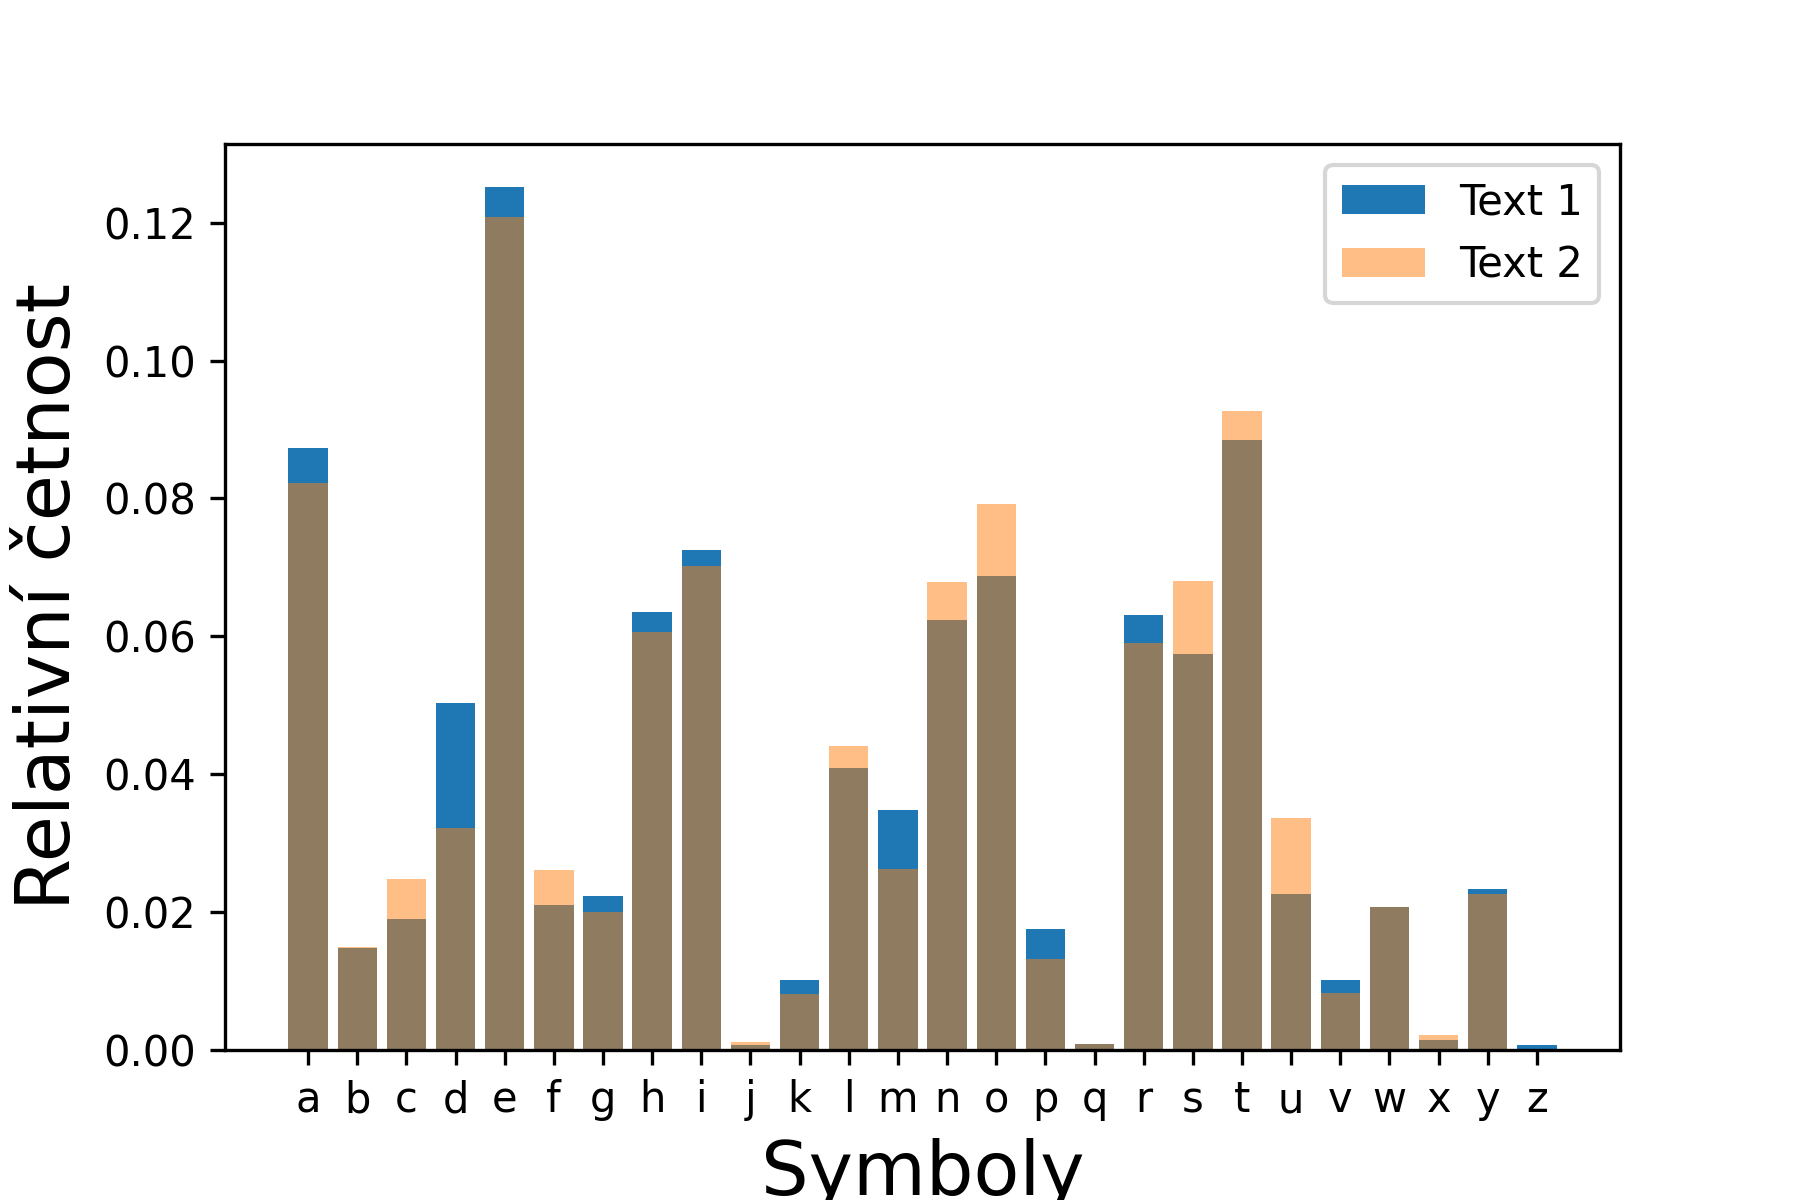
\includegraphics[width=1\columnwidth]{img/chdistr.png} 
\caption{Relativní četnosti písmen obou textů.}
\label{fig:chdistr}
\end{figure}

Pro úlohu č.2 jsme přemodelovali náhodné veličiny na četnosti znaků, což svým rozdělením odpovídá multinomickému rozdělení. Pravděpodobnosti písmen jsme odhadli jako relativní četnosti, tedy počet výskytů daného symbolu vydělený počtem všech symbolů. Tyto pravděpodobnosti jsou znázorněny na obrázku \ref{fig:chdistr}.

\section{Úloha č.3}
\textit{Na hladině významnosti 5\% otestujte hypotézu, že rozdělení délek slov nezávisí na tom, o který jde text. Určete také p-hodnotu testu.}\\
\begin{table*}[t]
\centering
\caption{Kontingenční tabulka třetí úlohy.}
\begin{tabular}{|r|rrrrrrrrrrr|r|} 
\hline
   & \multicolumn{1}{r|}{1} & \multicolumn{1}{r|}{2} & \multicolumn{1}{r|}{3} & \multicolumn{1}{r|}{4} & \multicolumn{1}{r|}{5} & \multicolumn{1}{r|}{6} & \multicolumn{1}{r|}{7} & \multicolumn{1}{r|}{8} & \multicolumn{1}{r|}{9} & \multicolumn{1}{r|}{10} & \multicolumn{1}{r|}{11+}  &$ \sum $       \\ 
\hline
005 & 68                     & 202                    & 251                    & 216                    & 106                    & 113                    & 51                     & 20                     & 26                     & 16                      & 11                         & 1080  \\
017 & 44                     & 251                    & 285                    & 216                    & 140                    & 128                    & 81                     & 50                     & 38                     & 20                      & 17                         & 1270  \\ 
\hline
  $ \sum $  & 112                    & 453                    & 536                    & 432                    & 246                    & 241                    & 132                    & 70                     & 64                     & 36                      & 28  & 2350  \\
\hline
\end{tabular}
\label{tab:3}
\end{table*}

Cílem třetí úlohy bylo rozhodnout zda rozdělení délek slov nezávisí na tom, o který jde text. Tedy jsme testovali, nezávislost mezi veličinami náhodného vektoru $ (X,Y)^T $, kde náhodná veličina $ X $ určuje číslo textu a $ Y $ délku slova. Tento vektor má diskrétní rozdělení. Na základě dat jsme sestavili kontingenční tabulku. Za nulovou hypotézu $ H_0 $ jsme postavili nezávislost těchto veličin, tedy $ H_0: p_{ij}=p_{i \bullet} p_{\bullet j} $, oproti alternativní hypotéze $ H_A: p_{ij}\neq p_{i \bullet} p_{\bullet j} $. Test nezávistlosti pomocí Pearsonovy statistiky $ \chi^2 $ jsme nemuseli dělat ručně, jelikož je součástí knihovny Scipy jako funkce \textit{chi2\_contingency}. Předtím než jsme provedli samotný test, bylo důležité zkontrolovat teoretické četnosti vypočítané z kontingenční tabulky pomocí funkce \textit{expected\_freq} ze stejné knihonvy. Testová statistika $ \chi^2 $ je pouze asymptotická, a při nizkých teoretických četnostech $ np_{ij} \leq 5 $ dává nepřesné výsledky. Vypočítané teoretické četnosti byly nedostačující u nejdelších slov. Jako řešení jsme tato slova počítali jako o písmeno kratší slova, dokud jsme nedosáhli požadovaných četností. Poté už jsme mohli použít zmíněnou funkci. Výstup funkce je testová statistika, p-hodnota, stupně volnosti a teoretické četnosti. Podle $ \hat{p} = 0.002 $ jsme zamítli nulovou hypotézu $ H_0 $ ve prospěch alternativní hypotézy $ H_A $. Pro jistotu jsme také spočítali kritickou hodnotu $ \chi^2_{\alpha,(r-1)(c-1)} $, kde $ \alpha = 0.05, r = 11 $ a $ c = 2 $. Dle očekávání platí $ \chi^2 \geq \chi^2_{0.05,10} $.

\begin{align*}
\chi^2 &= 26.7\\
\hat{p} &= 0.002\\
\chi^2_{0.05,10} &= 18.307
\end{align*}

\section{Úloha č.4}
\textit{Na hladině významnosti 5\% otestujte hypotézu, že se střední délky slov v obou textech rovnají. Určete také p-hodnotu testu.}\\

Ve čtvrté úloze jsme testovali hypotézu, zda se střední délky slov v obou textech rovnají. Jako nulovou hypotézu $ H_0 $ jsme postavili $ \mu_1 = \mu_2 $ oproti alternativní $ H_A: \mu_1 \neq \mu_2 $. 

\begin{align*}
H_0: \mu_1 = \mu_2\\
H_A: \mu_1 \neq \mu_2
\end{align*}

Pro tento týp úlohy je vhodný dvouvýběrový t-test. Předtím než tento test můžeme využít musíme zjistit, zda se rozptyly se rovnají nebo nerovnají. K tomu lze využít jiný test. Na základě nejistoty v normalitu $ X $ a $ Y $ jsme se rozhodli pro využití Levenova testu rovnosti rozptylů $ \sigma^2_1, \sigma^2_2 $, který je v tomto případě výhodnější. Za hladinu významnosti volíme 5\%.
\begin{align*}
W &= 4.838\\
\hat{p} &= 0.0279
\end{align*}
Dle p-hodnoty $ \hat{p} $, která je menší než zvolená hodnota $ \alpha $, můžeme zamítnout hypotézu $ H_0 $, ve prospěch $ H_A $, podle které se hodnoty rozptylů nerovnají. Toto můžeme ověřit nahlédnutím do úlohy 1, ve které jsme bodově odhadovali tyto rozptyly, kde se rozptyly opravdu nepodobají.
Na základě předchozího výsledku jsme již mohli využít spravný typ dvouvýběrového t-testu s rozdílnými rozptyly. V knihovně SciPy je pro tento test funkce \textit{ttest\_ind}, která nabízí parametr rovnosti rozptylů \textit{equal\_var}.
\begin{align*}
T &= -3.033\\
\hat{p} &= 0.00244
\end{align*}
Na základě $ \hat{p} $ jsme zamítli $ H_0 $ ve prospěch $ H_A $. Tedy střední délky slov obou textů se nerovnají.

\section{Úloha č.5}
\textit{Na hladině významnosti 5\% otestujte hypotézu, že rozdělení písmen nezávisí na tom, o který jde text. Určete také p-hodnotu testu.}\\

Podobně jako ve třetí úloze jsme v této úloze testovali nezávislost dvou veličin náhodného vektoru $ (X,Y)^T $, kde náhodná veličina $ X $ určuje číslo textu, ale $ Y $ již neurčuje délku slov, ale četnosti symbolů. Postupovali jsme velice podobně. Za nulovou hypotézu $ H_0 $ jsme postavili nezávislost těchto veličin, tedy $ H_0: p_{ij}=p_{i \bullet} p_{\bullet j} $, oproti alternativní hypotéze $ H_A: p_{ij}\neq p_{i \bullet} p_{\bullet j} $. Dále jsme na základě teoretických četností sestavili kontingenční tabulku tak, abychom mohli použít asymptotickou $ \chi^2 $ statistiku. Kvůli nedostatku četností pro písmena \textit{j, q, x, z}, jsme tyto písmena spojili do jednoho symbolu. Poté jsme opět využili funkci \textit{chi2\_contingency}.

\begin{align*}
\chi^2 &= 60.431\\
\hat{p} &= 1.9\times 10^{-5}\\
\chi^2_{0.05,22} &= 33.92
\end{align*}

Dle p-hodnoty jsme zamítli nulovou hypotézu ve prospěch té alternativní, říkající, že rozdělení písmen závisí na daném textu.

\end{document}
